\usetikzlibrary[positioning,fit,shadings]
\definecolor{bgblue}{rgb}{0.3,0.3,1}
\definecolor{bgred}{rgb}{1,0.3,0.3}
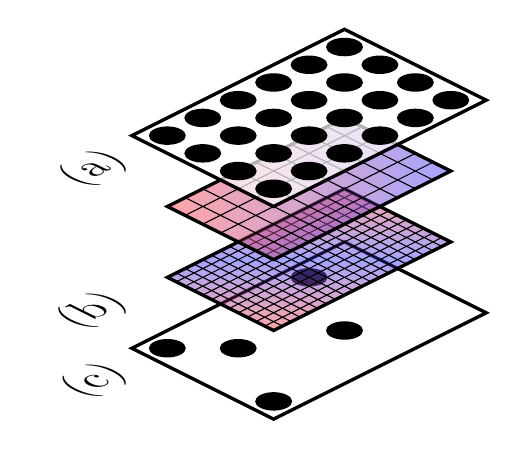
\begin{tikzpicture}[scale=0.45]

  \begin{scope}[shift={(0,-6)},every node/.append style={yslant=0.5,xslant=-1},yslant=0.5,xslant=-1](b)
    \foreach \x / \y in {0/0,1/2,3/1,4/3,0/3} {
      \foreach \lx / \ly in {0/0,1/2,3/1,4/3,0/3} {
        \drawLinewithBG{\x,\y}{\lx,\ly};
      }    
    }
    \foreach \x / \y in {0/0,1/2,3/1,4/3,0/3} {
      \node at (\x,\y) [circle,fill=black] (p/\x/\y) {};
    }
    \draw[black,very thick] (-0.5,-0.5) rectangle (5.5,3.5);
    \node at (-1,2) [label={[font=\Large](c)}] {};
  \end{scope}

  \begin{scope}[shift={(0,-4)},every node/.append style={yslant=0.5,xslant=-1},yslant=0.5,xslant=-1](b)
    \shade [top color=bgred, bottom color=bgred, middle color=bgblue,opacity=0.5] (0,0) rectangle (5,3);
    \draw[step=0.25,color=black] (0,0) grid (5,3);
    \draw[black,very thick] (0,0) rectangle (5,3);
    \node at (-1,2) [label={[font=\Large](b)}] {};
  \end{scope}
  
  \begin{scope}[shift={(0,-2)},every node/.append style={yslant=0.5,xslant=-1},yslant=0.5,xslant=-1](b)
    \shade[left color=bgred, middle color=bgblue, right color=bgblue,opacity=0.5](0,0) rectangle (5,3);
    \draw[step=0.5,color=black] (0,0) grid (5,3);
    \draw[black,very thick] (0,0) rectangle (5,3);
  \end{scope}

  
  \begin{scope}[yshift=0em,every node/.append style={yslant=0.5,xslant=-1},yslant=0.5,xslant=-1](a)
    \fill[white,fill opacity=0.7] (-0.5,-0.5) rectangle  (5.5,3.5);
    \foreach \x in {0,1,2,3,4,5} {
      \foreach \y in {0,1,2,3} {
        \node at (\x,\y) [circle,fill=black] (o/\x/\y) {};
      }
    }
    \draw[black,very thick] (-0.5,-0.5) rectangle (5.5,3.5);
    \node at (-1,2) [label={[font=\Large](a)}] {};
  \end{scope}

\end{tikzpicture}